\section{Numerical methods for overdetermined linear systems and SVD}

\subsection{Overdetermined systems and Least Squares}

An \definition{Overdetermined linear system} is a \textbf{system of linear equations in which there are more equations than unknowns}. In other words, there are more constraints than variables, which often makes it \emph{impossible to satisfy all the equations simultaneously}. This often happens in practical applications where we have more measurements or constraints than variables.

\highspace
The solution method is \definitionWithSpecificIndex{Least Squares}{Least Squares method}; it finds an approximate \textbf{solution by minimizing the sum of the squares of the residuals} (the differences between the left and right sides of the equations). A practical implementation is Singular Value Decomposition (SVD).

\highspace
\begin{flushleft}
    \textcolor{Green3}{\faIcon{square-root-alt} \textbf{Mathematical point of view}}
\end{flushleft}
The mathematical problem reads: given $A \in \mathbb{R}^{m \times n}$, with $m \ge n$ and $\mathbf{b} \in \mathbb{R}^{m}$, find $\mathbf{x} \in \mathbb{R}^{n}$ such that: $A\mathbf{x} = \mathbf{b}$.

\begin{figure}[!htp]
    \centering
    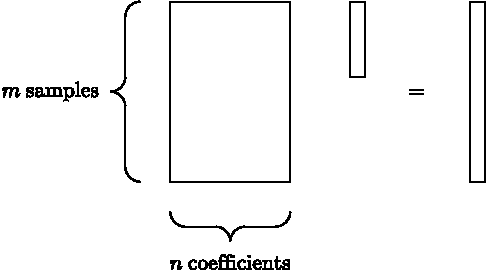
\includegraphics[width=.6\textwidth]{img/overdetermined-linear-systems-1.pdf}
\end{figure}

\noindent
Note that the above problems generally have no solution unless the right side $\mathbf{b}$ is an element of $\mathrm{range}\left(A\right)$ (all possible linear combinations of the columns of $A$). So the basic approach is to look for a $\mathbf{x}$ that makes $A\mathbf{x}$ \dquotes{close} to $\mathbf{b}$.

\highspace
We compute the solution using least-squares. Given $A \in \mathbb{R}^{m \times n}$, $m \ge n$, we say that $\mathbf{x}^{*} \in \mathbb{R}^{n}$ is a solution of the linear system $A\mathbf{x} = \mathbf{b}$ in the least-squares sense if:
\begin{equation}
    \Phi\left(\mathbf{x}^{*}\right) = \underset{\mathbf{y} \in \mathbb{R}^{n}}{\min} \Phi\left(\mathbf{y}\right)
\end{equation}
Where:
\begin{equation}
    \Phi\left(\mathbf{y}\right) = {\left|\left|A\mathbf{y} - \mathbf{b}\right|\right|}_{2}^{2}
\end{equation}
The problem thus consists of minimizing the Euclidean norm of the residual. The \textbf{solution} $\mathbf{x}^{*}$ can be \textbf{found by imposing the condition that the gradient of the function} $\Phi\left(\cdot\right)$ \textbf{must be equal to zero at} $\mathbf{x}^{*}$. From the definition we have:
\begin{equation*}
    \begin{array}{rcl}
        \Phi\left(\mathbf{y}\right) &=& \left(A\mathbf{y} - \mathbf{b}\right)^{T}\left(A\mathbf{y} - \mathbf{b}\right) \\ [.3em]
        %
        &=& \mathbf{y}^{T}A^{T}A\mathbf{y} - 2\mathbf{y}^{T} A \mathbf{b} + \mathbf{b}^{T}\mathbf{b}
    \end{array}
\end{equation*}
Therefore:
\begin{equation*}
    \nabla\Phi\left(\mathbf{y}\right) = 2A^{T} A \mathbf{y} - 2A^{T}\mathbf{b}
\end{equation*}
From which it follows that $\mathbf{x}^{*}$ must be the solution of the square system:
\begin{equation}
    A^{T}A\mathbf{x}^{*} = A^{T}\mathbf{b}
\end{equation}

\highspace
The system of normal equations is nonsingular if $A$ has \textbf{full rank} and, in such a case, the least-squares \textbf{solution exists and is unique}.

\begin{theorem}
    Let $A \in \mathbb{R}^{m \times n}$, with $m \ge n$, be a full rank matrix. Then the \textbf{unique solution} in the least-square sense $\mathbf{x}^{*}$ of $A\mathbf{x}^{*} = \mathbf{b}$ is given by $\mathbf{x}^{*} = \widehat{R}^{-1}\widehat{Q}^{T}\mathbf{b}$, where $\widehat{R} \in \mathbb{R}^{n \times n}$ and $\widehat{Q} \in \mathbb{R}^{m \times n}$ are the matrices of the reduced QR factorization of A. Moreover, the minimum of $\Phi\left(\cdot\right)$ is given by:
    \begin{equation*}
        \Phi\left(\mathbf{x}^{*}\right) = \displaystyle\sum_{i = n+1}^{m} \left[\left(Q^{T}b\right)_{i}\right]^{2}
    \end{equation*}
\end{theorem}

\noindent
If $A$ has full rank, then since the solution exists in the least squares sense and is unique, it must necessarily have \textbf{minimal Euclidean norm}:
\begin{equation}\label{eq: minimal Euclidean norm}
    {\left|\left|A \mathbf{x}^{*} - \mathbf{b}\right|\right|}_{2}^{2} \le \underset{\mathbf{x} \in \mathbb{R}^{n}}{\min} {\left|\left|A\mathbf{x} - \mathbf{b}\right|\right|}_{2}^{2}
\end{equation}

\highspace
In other words, given an overdetermined system $A\mathbf{x} = \mathbf{b}$, the least squares method finds $\mathbf{x}$ that minimizes the quantity ${\left|\left|A\mathbf{x} - \mathbf{b}\right|\right|}_{2}^{2}$. These problems can be solved using the SVD method.
